\mysection{Evaluation}
\label{sec:nate:evaluation}
\pgfplotstableset{col sep=comma}

% \pgfplotstableread{nate/data/sp14/op+type+size/linear/results.csv}{\FeatureLinearBench}
% \pgfplotstablevertcat{\FeatureLinearBench}{nate/data/sp14/op+context+type+size/linear/results.csv}
% \pgfplotstablevertcat{\FeatureLinearBench}{nate/data/sp14/op+context-has+type+size/linear/results.csv}
% \pgfplotstablevertcat{\FeatureLinearBench}{nate/data/sp14/op+context-count+type+size/linear/results.csv}
% \pgfplotstableread{nate/data/sp14/op+type+size/hidden-10/results.csv}{\FeatureHiddenTBench}
% \pgfplotstablevertcat{\FeatureHiddenTBench}{nate/data/sp14/op+context+type+size/hidden-10/results.csv}
% \pgfplotstablevertcat{\FeatureHiddenTBench}{nate/data/sp14/op+context-has+type+size/hidden-10/results.csv}
% \pgfplotstablevertcat{\FeatureHiddenTBench}{nate/data/sp14/op+context-count+type+size/hidden-10/results.csv}
% \pgfplotstableread{nate/data/sp14/op+type+size/hidden-500/results.csv}{\FeatureHiddenFHBench}
% \pgfplotstablevertcat{\FeatureHiddenFHBench}{nate/data/sp14/op+context+type+size/hidden-500/results.csv}
% \pgfplotstablevertcat{\FeatureHiddenFHBench}{nate/data/sp14/op+context-has+type+size/hidden-500/results.csv}
% \pgfplotstablevertcat{\FeatureHiddenFHBench}{nate/data/sp14/op+context-count+type+size/hidden-500/results.csv}

% \pgfplotstableread{nate/data/sp14/op+type+size/hidden-10/results.csv}{\HiddenBench}
% \pgfplotstablevertcat{\HiddenBench}{nate/data/sp14/op+type+size/hidden-25/results.csv}
% \pgfplotstablevertcat{\HiddenBench}{nate/data/sp14/op+type+size/hidden-50/results.csv}
% \pgfplotstablevertcat{\HiddenBench}{nate/data/sp14/op+type+size/hidden-100/results.csv}
% \pgfplotstablevertcat{\HiddenBench}{nate/data/sp14/op+type+size/hidden-250/results.csv}
% \pgfplotstablevertcat{\HiddenBench}{nate/data/sp14/op+type+size/hidden-500/results.csv}
% % \pgfplotstablevertcat{\HiddenBench}{nate/data/sp14/op+context-count+type+size/hidden-10/results.csv}
% % \pgfplotstablevertcat{\HiddenBench}{nate/data/sp14/op+context-count+type+size/hidden-25/results.csv}
% % \pgfplotstablevertcat{\HiddenBench}{nate/data/sp14/op+context-count+type+size/hidden-50/results.csv}
% % \pgfplotstablevertcat{\HiddenBench}{nate/data/sp14/op+context-count+type+size/hidden-100/results.csv}
% % \pgfplotstablevertcat{\HiddenBench}{nate/data/sp14/op+context-count+type+size/hidden-250/results.csv}
% % \pgfplotstablevertcat{\HiddenBench}{nate/data/sp14/op+context-count+type+size/hidden-500/results.csv}

\pgfplotstableread{nate/data/sp14/baseline.csv}{\SpringBench}
\pgfplotstablevertcat{\SpringBench}{nate/data/sp14/ocaml/results.csv}
\pgfplotstablevertcat{\SpringBench}{nate/data/sp14/mycroft/results.csv}
\pgfplotstablevertcat{\SpringBench}{nate/data/sp14/sherrloc/results.csv}
\pgfplotstablevertcat{\SpringBench}{nate/data/sp14/op+context+type+size/linear/results.csv}
\pgfplotstablevertcat{\SpringBench}{nate/data/sp14/op+context+type+size/decision-tree/results.csv}
\pgfplotstablevertcat{\SpringBench}{nate/data/sp14/op+context+type+size/random-forest/results.csv}
\pgfplotstablevertcat{\SpringBench}{nate/data/sp14/op+context+type+size/hidden-10/results.csv}
\pgfplotstablevertcat{\SpringBench}{nate/data/sp14/op+context+type+size/hidden-500/results.csv}

\pgfplotstableread{nate/data/fa15/baseline.csv}{\FallBench}
\pgfplotstablevertcat{\FallBench}{nate/data/fa15/ocaml/results.csv}
\pgfplotstablevertcat{\FallBench}{nate/data/fa15/mycroft/results.csv}
\pgfplotstablevertcat{\FallBench}{nate/data/fa15/sherrloc/results.csv}
\pgfplotstablevertcat{\FallBench}{nate/data/fa15/op+context+type+size/linear/results.csv}
\pgfplotstablevertcat{\FallBench}{nate/data/fa15/op+context+type+size/decision-tree/results.csv}
\pgfplotstablevertcat{\FallBench}{nate/data/fa15/op+context+type+size/random-forest/results.csv}
\pgfplotstablevertcat{\FallBench}{nate/data/fa15/op+context+type+size/hidden-10/results.csv}
\pgfplotstablevertcat{\FallBench}{nate/data/fa15/op+context+type+size/hidden-500/results.csv}

\pgfplotstableread{nate/data/models/linear-op+slice-no-slice.cross.csv}{\SliceLinearBench}
\pgfplotstablevertcat{\SliceLinearBench}{nate/data/models/linear-op+slice.cross.csv}
\pgfplotstablevertcat{\SliceLinearBench}{nate/data/models/linear-op+slice-only-slice.cross.csv}
\pgfplotstableread{nate/data/models/hidden-500-op+slice-no-slice.cross.csv}{\SliceHiddenBench}
\pgfplotstablevertcat{\SliceHiddenBench}{nate/data/models/hidden-500-op+slice.cross.csv}
\pgfplotstablevertcat{\SliceHiddenBench}{nate/data/models/hidden-500-op+slice-only-slice.cross.csv}
% \pgfplotstablecreatecol[create col/assign/.code={%
%     \edef\entry{\thisrow{features}/\thisrow{model}}
%     \pgfkeyslet{/pgfplots/table/create col/next content}\entry
%   }]{tool}{\SliceBench}

\pgfplotstableread{nate/data/models/linear-op.cross.csv}{\FeatureLinearBench}
\pgfplotstablevertcat{\FeatureLinearBench}{nate/data/models/linear-op+size.cross.csv}
\pgfplotstablevertcat{\FeatureLinearBench}{nate/data/models/linear-op+context.cross.csv}
\pgfplotstablevertcat{\FeatureLinearBench}{nate/data/models/linear-op+type.cross.csv}
\pgfplotstablevertcat{\FeatureLinearBench}{nate/data/models/linear-op+context+size.cross.csv}
\pgfplotstablevertcat{\FeatureLinearBench}{nate/data/models/linear-op+type+size.cross.csv}
\pgfplotstablevertcat{\FeatureLinearBench}{nate/data/models/linear-op+context+type.cross.csv}
\pgfplotstablevertcat{\FeatureLinearBench}{nate/data/models/linear-op+context+type+size.cross.csv}
\pgfplotstableread{nate/data/models/linear-op.cross.csv}{\FeatureHiddenBench}
\pgfplotstablevertcat{\FeatureHiddenBench}{nate/data/models/hidden-500-op+size.cross.csv}
\pgfplotstablevertcat{\FeatureHiddenBench}{nate/data/models/hidden-500-op+context.cross.csv}
\pgfplotstablevertcat{\FeatureHiddenBench}{nate/data/models/hidden-500-op+type.cross.csv}
\pgfplotstablevertcat{\FeatureHiddenBench}{nate/data/models/hidden-500-op+context+size.cross.csv}
\pgfplotstablevertcat{\FeatureHiddenBench}{nate/data/models/hidden-500-op+type+size.cross.csv}
\pgfplotstablevertcat{\FeatureHiddenBench}{nate/data/models/hidden-500-op+context+type.cross.csv}
\pgfplotstablevertcat{\FeatureHiddenBench}{nate/data/models/hidden-500-op+context+type+size.cross.csv}
% \pgfplotstablecreatecol[create col/assign/.code={%
%     \edef\entry{\thisrow{features}/\thisrow{model}}
%     \pgfkeyslet{/pgfplots/table/create col/next content}\entry
%   }]{tool}{\FeatureBench}


We have implemented our technique for localizing type errors for a
purely functional subset of \ocaml with polymorphic types and functions.
%
We seek to answer four questions in our evaluation:
%
\begin{itemize}
\item \textbf{Blame Accuracy}
  %
  How often does \toolname
  blame a \emph{correct}
  location for the error?
  (\autoref{sec:nate:quantitative})
  %
  % We compare our technique with a variety of off-the-shelf classifiers
  % and find that our top-ranked blame assignments have an accuracy of
  % 72\%, compared to a state-of-the-art 56\%.
  % For how many ill-typed programs can we accurately predict the source
  % of the error?
\item \textbf{Feature Utility}
  %
  Which program \emph{features are required}
  to localize errors?
   (\autoref{sec:nate:feature-utility})
  % How much do the features described in \autoref{sec:nate:features}
  % contribute to our predictions?
\item \textbf{Interpretability}
  %
  %% Do the models learned by \toolname
  %% correspond to our intuition about
  %% the real causes of errors?
  Do the models match our intuition about type errors?
  (\autoref{sec:nate:qualitative})
\item \textbf{Blame Utility}
  Do \toolname's blame assignments help
  users diagnose type errors?
  (\autoref{sec:nate:user-study})
\end{itemize}
%
%\paragraph{Summary of Results}
%
In the sequel we present our experimental
methodology \autoref{sec:nate:methodology} and
then drill into how we evaluated each of
the questions above.
%
However, for the impatient reader, we begin
with a quick summary of our main results:
%
%
%\begin{itemize}
%
%\item \textbf

\paragraph{1. Data Beats Algorithms}
Our main result is that for type error
localization, data is indeed unreasonably
effective \citep{Halevy2009-so}.
%
When trained on student errors from one
instance of an undergraduate course and
tested on another instance,
\toolname's most sophisticated
\emph{neural network}-based
classifier's top-ranked
prediction blames the correct
sub-term \HiddenFhTopOne\% of the time
--- a good \ToolnameWinSherrloc points
higher than the state-of-the-art
\sherrloc's \SherrlocTopOne\%.
%
However, even \toolname's simple
\emph{logistic regression} based
classifier is correct \LinearTopOne\% of the time,
\ie \LinearWinSherrloc points better than \sherrloc.
%
When the top three predictions are considered,
\toolname is correct \HiddenFhTopThree\% of the time.

% \item \textbf
\paragraph{2. Slicing Is Critical}
%
However, data is effective \emph{only}
when irrelevant sub-terms have been
sliced out of consideration.
%
In fact, perhaps our most surprising
result is that type error slicing and
local syntax alone yields
a classifier that is \SlicingWinOcaml points
better than \ocaml and on par with
\sherrloc.
%
That is, once we focus our classifiers on
slices, purely local syntactic features
perform as well as the
state-of-the-art.

%\item \textbf
\paragraph{3. Size Doesn't Matter, Types Do}
%
We find that (after slices)
typing features
provide the biggest
improvement in accuracy.
%
Furthermore, we find contextual syntactic
features to be mostly (but not entirely)
redundant with typing features,
which supports the hypothesis that
the context's \emph{type} nicely
summarizes the properties of the
surrounding expressions.
%
Finally, we found that the \emph{size}
of the sub-expression was not very useful.
This was unexpected, as we thought
smaller expressions would be simpler, and
hence, more likely causes.

% \item \textbf
\paragraph{4. Models Learn Typing Rules}
%
Finally, by investigating a few of the
predictions made by the \emph{decision tree}-based
models, we found that the models
appear to capture some simple and intuitive
rules for predicting well-typedness.
%
For example, if the left child of an application
is a function, then the application is likely
correct.

% in an application, if the
% left argument is a function then the
% error is likely on the right sub-term;
% in a function definition
% \RJ{fixme: orig
% defining a function is a fine thing
% to do?}
%
%\end{itemize}
% \RJ{eric please check the numbers -- we say 71, 72, 74, 91, 92, 94?}


\mysubsection{Methodology}
\label{sec:nate:methodology}
We answer our questions on the two datasets gathered in
\autoref{chp:data-collection}, which we will briefly describe
again.
% We answer our questions on two sets of data gathered from the
% undergraduate Programming Languages course at
% % \begin{anonsuppress}
% UC San Diego (IRB \#140608).
% \end{anonsuppress}
% \begin{noanonsuppress}
% AUTHOR's INSTITUTION.
% \end{noanonsuppress}
%
We recorded each interaction with the \ocaml top-level system while
students in our undergraduate Programming Languages course
worked on 23 programs from the first three homework
assignments, capturing ill-typed programs and, crucially, their
subsequent fixes.
%
The first dataset comes from the Spring 2014 class (\SPRING), with a
cohort of 46 students. The second comes from the Fall 2015 class
(\FALL), with a cohort of 56 students.
%
The extracted programs are relatively small, but they demonstrate a
range of functional programming idioms, \eg higher-order functions and
(polymorphic) algebraic data types.

\paragraph{Feature Selection}
We extract 282 features from each sub-expression in a
program, including:
%
\begin{enumerate}
\item 45 local syntactic features. In addition to the syntax of \lang,
  we support the full range of arithmetic operators (integer and
  floating point), equality and comparison operators, character and
  string literals, and a user-defined % |expr| type of simple
  arithmetic
  expressions. We discuss the challenge of supporting other
  % user-defined
  types in \autoref{sec:nate:discussion}.
\item 180 contextual syntactic features. For each sub-expression we
  additionally extract the local syntactic features of its parent and
  first, second, and third (left-to-right) children. If an expression
  does not have a parent or children, these features will simply be
  disabled. If an expression has more than three children, the
  classifiers will receive no information about the additional
  children.
\item 55 typing features. In addition to the types of \lang, we support
  |int|s, |float|s, |char|s, |string|s, and the user-defined |expr|
  mentioned above. These features are extracted for each sub-expression
  and its context. % for the contextual sub-expressions.
\item One feature denoting the size of each sub-expression.
\item One feature denoting whether each sub-expression is part of the
  minimal type error slice. We use this feature as a ``hard''
  constraint, sub-expressions that are not part of the minimal slice
  will be preemptively discarded. We justify this decision in
  \autoref{sec:nate:feature-utility}.
\end{enumerate}

\paragraph{Blame Oracle}
Recall from \autoref{sec:nate:labels} that we automatically extract a blame
oracle for each ill-typed program from the (AST) diff between it and the
student's eventual fix.
%
A disadvantage of using diffs in this manner is that students may have
made many, potentially unrelated, changes between compilations; at some
point the ``fix'' becomes a ``rewrite''.
%
We do not wish to consider the ``rewrites'' in our evaluation, so we
discard outliers where the fraction of expressions that have changed is
more than one standard deviation above the mean, establishing a diff
threshold of 40\%.
%
This accounts for roughly 14\% of each dataset, leaving us with
2,712 program pairs for \SPRING and 2,365 pairs for \FALL.

% we discard any program pairs where more than 40\%
% of the sub-expressions have changed.
% %
% We picked 40\% as an estimate of the inflection point where we could
% still retain the large majority of program pairs.
% % FIXME: Can you say that this dataset curation is similar to any other
% % datasets (e.g., the washington one)? Anything you could cite and discuss
% % here would take some of the pressure off.


\paragraph{Accuracy Metric}
All of the tools we compare (with the exception of the standard \ocaml
compiler) can produce a list of potential error locations.
%
However, in a study of fault localization techniques,
\citet{Kochhar2016-oc} show that most developers will not consider more
than around five potential error locations before falling back to manual
debugging.
%
Type errors are relatively simple in comparison to general fault
localization, thus we limit our evaluation to the top three predictions
of each tool.
%
We evaluate each tool on whether a changed expression occurred in its
top one, top two, or top three predictions.

\mysubsection{Threats to Validity}
\label{sec:nate:validity}

Although our experiments demonstrate that our technique can pinpoint type
errors more accurately than the state of the art and that our features are
relevant to blame assignment, our results may not generalize.

One threat to validity associated with supervised machine learning is
overfitting (\ie learning a model that is too complex with respect to
the data).
%
A similar issue that arises in machine learning is model stability (\ie
can small changes to the training set produce large changes in the model?).
%
We mitigate these threats by:
%
(1) using separate training and testing datasets drawn from distinct
student populations (\autoref{sec:nate:quantitative}), demonstrating the
generality of our models; and
%
(2) via cross-validation on the joint dataset
(\autoref{sec:nate:feature-utility}), which demonstrates the stability of our
models by averaging the accuracy of 10 models trained on distinct
subsets of the data.

Our benchmarks were drawn from students in an undergraduate course and
may not be representative of other student populations.
%
We mitigate this threat by including the largest empirical evaluation of
type error localization that we are aware of: over 4,500 pairs of
ill-typed programs and fixes from two instances of the course, with
programs from 102 different students.
%
We acknowledge, of course, that students are not industrial programmers
and our results may not translate to large-scale software development;
however, we are particularly interested in aiding novice programmers
as they learn to work inside the type system.

A related threat to construct validity is our definition of the immedate
next well-typed program as the intended ground truth answer (see
\autoref{sec:nate:overview}, Challenge 2). Students may, in theory, submit
intermediate well-typed program ``rewrites'' between the original ill-typed
program and the final intended answer. Our approach to discarding outliers
(see \autoref{sec:nate:evaluation}) is designed to mitigate this threat.

Our removal of program pairs that changed too much, where our oracle
could not identify the blame of the other tools, or where the other
tools timed out or encountered unsupported language features is another
threat to validity.
%
It is possible that including the programs that changed excessively
would hurt our models, or that the other tools would perform
better on the programs with unsupported language features.
%
We note however that
%
(1) outlier removal is a standard technique in machine learning%
%\ES{CITE?}
; and
%
(2) our Top-1 accuracy margin is large enough that even if we assumed
that \sherrloc were perfect on all excluded programs,
% it would only tie our \hiddenFH. % in Top-1 accuracy.
we would still lead by 10 points.
%
%\ES{I think this is accurate, but should double check..}

Examining programs written in \ocaml as opposed to \haskell or any other
typed functional language poses yet another threat, common type errors
may differ in different languages.
%
\ocaml is, however, a standard target for research in type error
localization and thus our choice admits a direct comparison with prior
work.
%
Furthermore, the functional core of \ocaml that we support does not
differ significantly from the functional core of \haskell or SML, all of
which are effectively lambda calculi with a Hindley-Milner-style type
system.
% \footnote{\haskell's type classes are a notable exception, they
%   are also known to cause confusing type errors and would be interesting
%   to study as well.}

Finally, our use of student fixes as oracles
% for the source of type errors
assumes that students are able to correctly identify
the source of an error.
%
As the students are in the process of learning the language and type
system, this assumption may be faulty.
%
It may be that \emph{expert} users would disagree with many of the
student fixes, and that it is harder to learn a model of expert fixes,
or that the state of the art would be better at predicting expert fixes.
%
As we have noted before, we believe it is reasonable to use student
fixes as oracles because the student is the best judge of what she
\emph{intended}.


\mysubsection{Blame Accuracy}
\label{sec:nate:quantitative}

First, we compare the accuracy of our predictions to the
state of the art in type error localization.

\mypara{Baseline}
We provide two baselines for the comparison: a random choice of location
from the minimized type error slice, and the standard \ocaml compiler.

\mypara{State of the Art}
\mycroft~\citep{Loncaric2016-uk} localizes type errors by searching for
a minimal subset of typing constraints that can be removed, such that
the resulting system is satisfiable.
%
When multiple such subsets exist it can enumerate them, though it has no
notion of which subsets are \emph{more likely} to be correct, and thus
the order is arbitrary.
%
\sherrloc~\citep{Zhang2014-lv} localizes errors by searching the typing
constraint graph for constraints that participate in many unsatisfiable
paths and comparatively few satisfiable paths.
%
It can also enumerate multiple predictions, in descending order of
likelihood.

Comparing source locations from multiple tools with their own parsers is
not trivial.
%
Our experimental design gives the state of the art tools the ``benefit
of the doubt'' in two ways.
% To ensure a fair comparison when evaluating \mycroft and
% \sherrloc,
First, when evaluating \mycroft and \sherrloc, we did not consider
programs where they predicted locations that our oracle could not match
with a program expression: around 6\% of programs for \mycroft and 4\%
for \sherrloc.
%
Second, we similarly ignored programs where \mycroft or \sherrloc timed
out (after one minute) or where they encountered an unsupported language
feature: another 5\% for \mycroft and 12\% for \sherrloc.
%

\mypara{Our Classifiers}
We evaluate five classifiers, each trained on the full feature set.
% features: 44 local syntactic features, 176 contextual syntactic
% features, 55 typing features, and a single expression size feature.
% %
% \ES{should explain the make-up of these groups}
%
% We preemptively discard expressions that are not part of the minimal
% type error slice --- we will explain the rationale for this in
% \autoref{sec:nate:feature-utility} --- and thus the final feature count is
% 276.
%
These include:
%Our classifiers are:
%
\begin{description}
\item[\linear] A logistic regression trained with a learning rate
  $\eta = 0.001$, an $L_2$ regularization rate $\lambda = 0.001$, and a
  mini-batch size of 200.
\item[\dectree] A decision tree trained with the CART algorithm
  \citep{Breiman1984-qy} and an impurity threshold of $10^{-7}$ (used to
  avoid overfitting via early stopping).
\item[\forest] A random forest \citep{Breiman2001-wo} of 30
  estimators, with an impurity threshold of $10^{-7}$.
\item[\hiddenT and \hiddenFH] Two multi-layer perceptron neural
  networks, both trained with $\eta = 0.001$, $\lambda = 0.001$, and a
  mini-batch size of 200.
  %
  The first MLP contains a single hidden layer of 10 neurons, and the
  second contains a hidden layer of 500 neurons.
  %
  This gives us a measure of the complexity of the MLP's model, \ie
  if the model requires many compound features, one would expect \hiddenFH
  to outperform \hiddenT.
  % This allows us to investigate how well the MLP can \emph{compress} its
  % model (cf.~\cite{FIXME}).
  %
  The neurons use rectified linear units (ReLU) as their activation
  function, a common practice in modern neural networks.
\end{description}
%
All classifiers were trained for 20 epochs on one dataset
--- \ie they were shown each program 20 times ---
before being evaluated on the other.
%
The logistic regression and MLPs were trained with the \textsc{Adam}
optimizer \citep{Kingma2014-ng}, a variant of stochastic gradient
descent that has been found to converge faster.


% colors from http://colorbrewer2.org/?type=sequential&scheme=Blues&n=3
\definecolor{blue1}{HTML}{DEEBF7}
\definecolor{blue2}{HTML}{9ECAE1}
\definecolor{blue3}{HTML}{3182BD}
\definecolor{green1}{HTML}{E5F5E0}
\definecolor{green2}{HTML}{A1D99B}
\definecolor{green3}{HTML}{31A354}

% \begin{figure}[ht]
% \centering
% \begin{tikzpicture}
% \begin{axis}[
%   % ybar stacked,
%   width=12cm,
%   height=8cm,
%   title={Impact of Feature Set on Accuracy},
%   ylabel={Accuracy},
%   %ymin=0.2,
%   ymax=1,
%   yticklabel={\pgfmathparse{\tick*100}\pgfmathprintnumber{\pgfmathresult}\,\%},
%   ytick style={draw=none},
%   ymajorgrids = true,
%   symbolic x coords={op+type+size, op+context+type+size, op+context-has+type+size, op+context-count+type+size},
%   % enlarge x limits=0.25,
%   xtick=data,
%   xtick style={draw=none},
%   xticklabels={Type, Context-Is, Context-Has, Context-Count},
%   x tick label style={rotate=45},
%   reverse legend,
%   transpose legend,
%   legend style={legend pos = outer north east, legend columns=4},
% ]
% % \addplot[draw=black, fill=blue1] table[x=tool, y=top-1] {\HiddenBench};
% % \addplot[draw=black, fill=blue2] table[x=tool, y expr=\thisrow{top-2} - \thisrow{top-1}] {\HiddenBench};
% % \addplot[draw=black, fill=blue3] table[x=tool, y expr=\thisrow{top-3} - \thisrow{top-2}] {\HiddenBench};

% \addplot[mark options={fill=blue1, scale=1.5}, mark=square*]
%   table[x=features, y=top-1] {\FeatureHiddenFHBench};
% \addplot[mark options={fill=blue2, scale=1.5}, mark=square*]
%   table[x=features, y=top-2] {\FeatureHiddenFHBench};
% \addplot[mark options={fill=blue3, scale=1.5}, mark=square*]
%   table[x=features, y=top-3] {\FeatureHiddenFHBench};
% \addlegendentry{Top-1}
% \addlegendentry{Top-2}
% \addlegendentry{Top-3}
% \addlegendimage{empty legend}
% \addlegendentry{\hiddenFH}

% \addplot[mark options={fill=blue1, scale=1.5}, mark=*]
%   table[x=features, y=top-1] {\FeatureLinearBench};
% \addplot[mark options={fill=blue2, scale=1.5}, mark=*]
%   table[x=features, y=top-2] {\FeatureLinearBench};
% \addplot[mark options={fill=blue3, scale=1.5}, mark=*]
%   table[x=features, y=top-3] {\FeatureLinearBench};
% \addlegendentry{Top-1}
% \addlegendentry{Top-2}
% \addlegendentry{Top-3}
% \addlegendimage{empty legend}
% \addlegendentry{\linear}

% \end{axis}
% \end{tikzpicture}
% \caption{reuslts!}
% \label{fig:results}
% \end{figure}

% \begin{figure}[ht]
% \centering
% \begin{tikzpicture}
% \begin{axis}[
%   ybar stacked,
%   width=12cm,
%   height=8cm,
%   title={Impact of Hidden Layer Size on Accuracy},
%   ylabel={Accuracy},
%   bar width=20pt,
%   %ymin=0.2,
%   ymax=1,
%   yticklabel={\pgfmathparse{\tick*100}\pgfmathprintnumber{\pgfmathresult}\,\%},
%   ytick style={draw=none},
%   ymajorgrids = true,
%   symbolic x coords={op+type+size/hidden-10, op+type+size/hidden-25, op+type+size/hidden-50,
%                      op+type+size/hidden-100, op+type+size/hidden-250, op+type+size/hidden-500},
%   % enlarge x limits=0.25,
%   xtick=data,
%   xtick style={draw=none},
%   xticklabels={\hiddenT, \hiddenTF, \hiddenF, \hiddenH, \hiddenTHF, \hiddenFH},
%   x tick label style={rotate=45},
%   reverse legend,
%   legend style={legend pos = north west},
% ]
% \addplot[draw=black, fill=blue1] table[x=tool, y=top-1] {\HiddenBench};
% \addplot[draw=black, fill=blue2] table[x=tool, y expr=\thisrow{top-2} - \thisrow{top-1}] {\HiddenBench};
% \addplot[draw=black, fill=blue3] table[x=tool, y expr=\thisrow{top-3} - \thisrow{top-2}] {\HiddenBench};
% % \addplot[draw=black, fill=blue1] table[x=tool, y=top-1] {\HiddenBench};
% % \addplot[draw=black, fill=blue2] table[x=tool, y=top-2] {\HiddenBench};
% % \addplot[draw=black, fill=blue3] table[x=tool, y=top-3] {\HiddenBench};
% \legend{Top-1, Top-2, Top-3}
% \end{axis}
% \end{tikzpicture}
% \caption{reuslts!}
% \label{fig:results}
% \end{figure}

\begin{figure}[t]
\centering
\begin{tikzpicture}
\begin{axis}[
  ybar stacked,
  width=14cm,
  height=6cm,
  title={Accuracy of Type Error Localization Techniques},
  ylabel={Accuracy},
  bar width=0.5cm,
  ymin=0.2,
  ymax=1,
  ytick={0.2, 0.3, 0.4, 0.5, 0.6, 0.7, 0.8, 0.9, 1.0},
  yticklabel={\pgfmathparse{\tick*100}\pgfmathprintnumber{\pgfmathresult}\,\%},
  ytick style={draw=none},
  ymajorgrids = true,
  symbolic x coords={baseline, ocaml, mycroft, sherrloc,
                     op+context+type+size/linear,
                     op+context+type+size/decision-tree,
                     op+context+type+size/random-forest,
                     op+context+type+size/hidden-10,
                     op+context+type+size/hidden-500},
  %enlarge x limits=0.07,
  xtick=data,
  xtick style={draw=none},
  xticklabels={\random, \ocaml, \mycroft, \sherrloc,
               \linear, \dectree, \forest, \hiddenT, \hiddenFH},
  x tick label style={rotate=45, anchor=north east},
  %x tick label style={font=\small},
  y tick label style={font=\small},
  reverse legend,
  transpose legend,
  legend style={legend pos = north west, legend columns=4, font=\footnotesize},
]

% ES: NOTE: ORDER OF PLOTS/LEGEND ENTRIES MATTERS

\addplot[draw=black, fill=green1, bar shift=.25cm] table[x=tool, y=top-1] {\FallBench};
\addlegendentry{Top-1}
\addplot[draw=black, fill=green2, bar shift=.25cm] table[x=tool, y expr=\thisrow{top-2} - \thisrow{top-1}] {\FallBench};
\addlegendentry{Top-2}
\addplot[draw=black, fill=green3, bar shift=.25cm] table[x=tool, y expr=\thisrow{top-3} - \thisrow{top-2}] {\FallBench};
\addlegendentry{Top-3}
\addlegendimage{empty legend}
\addlegendentry{\FALL}

\resetstackedplots

\addplot[draw=black, fill=blue1, bar shift=-.25cm] table[x=tool, y=top-1] {\SpringBench};
\addlegendentry{Top-1}
\addplot[draw=black, fill=blue2, bar shift=-.25cm] table[x=tool, y expr=\thisrow{top-2} - \thisrow{top-1}] {\SpringBench};
\addlegendentry{Top-2}
\addplot[draw=black, fill=blue3, bar shift=-.25cm] table[x=tool, y expr=\thisrow{top-3} - \thisrow{top-2}] {\SpringBench};
\addlegendentry{Top-3}
\addlegendimage{empty legend}
\addlegendentry{\SPRING}


%\legend{Top-1, Top-2, Top-3}
\end{axis}
\end{tikzpicture}
\caption[Results of our comparison of type error localization
  techniques.]{
  %
  Results of our comparison of type error localization
  techniques.
  %
  We evaluate all techniques separately on two cohorts of
  students from different instances of an undergraduate
  Programming Languages course.
  %
  Our classifiers were trained on one cohort and evaluated on the other.
  %
  All of our classifiers outperform the state-of-the-art techniques
  \mycroft and \sherrloc.%  by a 10--15\% margin in Top-1 accuracy (with
%   the exception of \linear which is only slightly better than \sherrloc).
%
}
\label{fig:accuracy-results}
\end{figure}


\mypara{Results}
\autoref{fig:accuracy-results} shows the results of our experiment.
%
Localizing the type errors in our benchmarks amounted, on average, to
selecting one of 3 correct locations out of a slice of 10.
%
Our classifiers consistently outperform the competition, ranging from
\LinearTopOne\% Top-1 accuracy (\LinearTopThree\% Top-3)
for the \linear classifier to
\HiddenFhTopOne\% Top-1 accuracy (\HiddenFhTopThree\% Top-3)
for the \hiddenFH.\@
%
Our baseline of selecting at random achieves \BaselineTopOne\% Top-1
accuracy (\BaselineTopThree\% Top-3),
while \ocaml achieves a Top-1 accuracy of \OcamlTopOne\%.
%
Interestingly, one only needs two \emph{random} guesses to outperform
\ocaml, with \BaselineTopTwo\% accuracy.
%
\sherrloc outperforms both baselines, and comes close to our \linear classifier,
with \SherrlocTopOne\% Top-1 accuracy (\SherrlocTopThree\% Top 3),
while \mycroft underperforms \ocaml at \MycroftTopOne\% Top-1 accuracy.
%
% Finally, we find that \emph{all} of our classifiers outperform \sherrloc,
% ranging from 58--62\% Top-1 accuracy (86--88\% Top-3) for the \linear
% classifier to 71--74\% Top-1 accuracy (91\% Top-3) for the \hiddenFH.

Surprisingly, there is little variation in accuracy between our
classifiers.
%
With the exception of the \linear model, they all achieve around 70\%
Top-1 accuracy and around 90\% Top-3 accuracy.
%
This suggests that the model they learn is relatively simple.
%
In particular, notice that although the \hiddenT has $50\times$ \emph{fewer}
hidden neurons than the \hiddenFH, it only loses around 4\% accuracy.
% In particular, notice that the \hiddenT only loses around 2\% accuracy
% compared to the \hiddenFH,
%
We also note that our classifiers consistently perform better when
trained on the \FALL programs and tested on the \SPRING programs than
vice versa.
% , they appear to generalize better from the \FALL data.
% FIXME: Why? What is your explanation for this? Is it just sizes of those
% datasets or something qualitative about the program pairs in them?

\mysubsection{Feature Utility}
\label{sec:nate:feature-utility}
We have shown that we can train a classifier to effectively localize
type errors, but which of the feature classes from
\autoref{sec:nate:features} are contributing the most to our accuracy?
%
We focus specifically on feature \emph{classes} rather than individual
features as our 282 features are conceptually grouped into a much
smaller number of \emph{categorical} features.
%
For example, the syntactic class of an expression is conceptually a
feature but there are 45 possible values it could take; to encode this
feature for learning we split it into 45 distinct binary features.
%
Analyses that focus on individual features, \eg \textsc{ANOVA},
are difficult to interpret in our setting, as they will tell us the
importance of the binary features but not the higher-level categorical
features.
%
Thus, to answer our question we investigate the performance of
classifiers trained on various subsets of the feature classes.

\mysubsubsection{Type Error Slice}
\label{sec:nate:type-error-slice}
First we must justify our decision to automatically exclude expressions
outside the minimal type error slice from consideration.
%
% The \InSlice feature should be highly predictive --- a fix must change
% at least one expression in the type error slice.
% %
% Thus, our first experiment seeks to quantify the impact of \InSlice by
% comparing the accuracy of our classifiers on three sets of features:
%
Thus, we compare our classifiers on three sets of features:
%
\begin{enumerate}
\item A baseline with only local syntactic features and no
  preemptive filtering by \InSlice.
\item The features of (1) extended with \InSlice.
\item The same features as (1), but we preemptively discard samples
  where \InSlice is disabled.
\end{enumerate}
%
The key difference between (2) and (3) is that a classifier for (2) must
\emph{learn} that \InSlice is a strong predictor.
%
In contrast, a classifier for (3) must only learn about the syntactic
features, the decision to discard samples where \InSlice is disabled has
already been made by a human.
%
This has a few additional advantages: it reduces the set of candidate
locations by a factor of 7 on average, and it guarantees that any
prediction made by the classifier can fix the type error.
%
We expect that (2) will perform better than (1) as it contains more
information, and that (3) will perform better than (2) as the classifier
does not have to learn the importance of \InSlice.

% FIXME: Wes feels that there should be a sentence in the next mypara
% explaining to the reader why we didn't just use an ANOVA or the ReliefF
% method or whatever to figure out feature importance. Feature overlap?

We tested our hypothesis with the \linear and
%
\hiddenFH\footnote{A layer of 500 neurons is excessive when we have so few
  input features --- we use \hiddenFH for continuity with the
  surrounding sections.}
%
classifiers, cross-validated ($k=10$) over the combined SP14/FA15
dataset.
% We used a learning rate $\eta=0.001$, $L_2$ regularization rate
%$\lambda=0.001$, and mini-batch size of 200.
%
We trained for a single epoch on feature sets (1) and (2), and for 8
epochs on (3), so that the total number of training samples would be
roughly equal for each feature set.
%
\lstDeleteShortInline{|} % sigh...
In addition to accuracy, we report each
classifier's \emph{recall} --- \ie ``How many true changes can we
remember?'' --- defined as
$$
\frac{|\mathsf{predicted} \cap \mathsf{oracle}|}
     {|\mathsf{oracle}|}
$$
where $\mathsf{predicted}$ is limited to the top 3 predictions, and
$\mathsf{oracle}$ is the student's fix, limited to changes that are in
the type error slice.
%
We make the latter distinction as:
%
(1) changes that are not part of the type error slice are noise in the
data set; and
%
(2) it makes the comparison easier to interpret since $\mathsf{oracle}$
never changes.
% NOTE: keep this at the end of the para or it screws up spacing...
\lstMakeShortInline{|}
%
\begin{figure}[t]
\centering
\begin{subfigure}[t]{\linewidth}
\centering
\begin{tikzpicture}
\begin{axis}[
  name=slice,
  % scale only axis,
  %at=(feature.above north), anchor=below south east,
  ybar stacked,
  width=0.5\linewidth,
  height=4cm,
  %title={Impact of Type Error Slice},
  ylabel={Accuracy},
  bar width=0.5cm,
  ymin=0.2,
  ymax=1,
  ytick={0.2, 0.3, 0.4, 0.5, 0.6, 0.7, 0.8, 0.9, 1.0},
  yticklabel={\pgfmathparse{\tick*100}\pgfmathprintnumber{\pgfmathresult}\,\%},
  ytick style={draw=none},
  ymajorgrids = true,
  symbolic x coords={op+slice-no-slice, op+slice, op+slice-only-slice},
  enlarge x limits=0.25,
  xtick=data,
  xtick style={draw=none},
  xticklabels={\textsc{Local Syntax}, +\InSlice, \textsc{Filter \InSlice}},
  x tick label style={font=\small},
  y tick label style={font=\small},
  reverse legend,
  transpose legend,
  legend style={
    %legend pos = outer north east,
    at={(1.75,0.5)},
    anchor=center,
    legend columns=5
  },
]

% ES: NOTE: ORDER OF PLOTS/LEGEND ENTRIES MATTERS

\addplot+[stack plots=false, draw=black, fill=none, thick, bar shift=.25cm] table[x=features, y=recall] {\SliceHiddenBench};
\addlegendentry{Recall}
\addplot[draw=black, fill=green1, bar shift=.25cm] table[x=features, y=top-1] {\SliceHiddenBench};
\addlegendentry{Top-1}
\addplot[draw=black, fill=green2, bar shift=.25cm] table[x=features, y expr=\thisrow{top-2} - \thisrow{top-1}] {\SliceHiddenBench};
\addlegendentry{Top-2}
\addplot[draw=black, fill=green3, bar shift=.25cm] table[x=features, y expr=\thisrow{top-3} - \thisrow{top-2}] {\SliceHiddenBench};
\addlegendentry{Top-3}
\addlegendimage{empty legend}
\addlegendentry{\hiddenFH}

\resetstackedplots

\addplot+[stack plots=false, draw=black, fill=none, thick, bar shift=-.25cm] table[x=features, y=recall] {\SliceLinearBench};
\addlegendentry{Recall}
\addplot[draw=black, fill=blue1, bar shift=-.25cm] table[x=features, y=top-1] {\SliceLinearBench};
\addlegendentry{Top-1}
\addplot[draw=black, fill=blue2, bar shift=-.25cm] table[x=features, y expr=\thisrow{top-2} - \thisrow{top-1}] {\SliceLinearBench};
\addlegendentry{Top-2}
\addplot[draw=black, fill=blue3, bar shift=-.25cm] table[x=features, y expr=\thisrow{top-3} - \thisrow{top-2}] {\SliceLinearBench};
\addlegendentry{Top-3}
\addlegendimage{empty legend}
\addlegendentry{\linear}
\end{axis}
\begin{axis}[
  ybar stacked,
  width=0.5\linewidth,
  height=4cm,
  ylabel={Recall},
  axis y line*=right,
  ymin=0.2,
  ymax=1,
  ytick={0.2, 0.3, 0.4, 0.5, 0.6, 0.7, 0.8, 0.9, 1.0},
  yticklabel={\pgfmathparse{\tick*100}\pgfmathprintnumber{\pgfmathresult}\,\%},
  ytick style={draw=none},
  ymajorgrids = false,
  xmin=0, xmax=1,
  hide x axis,
]
\end{axis}
\end{tikzpicture}
\caption{Impact of type error slice on blame accuracy.}\label{fig:slice-utility}
\end{subfigure}

%\hfill\mbox{}

\vspace{1\baselineskip}


\begin{subfigure}[t]{\linewidth}
\begin{tikzpicture}
\begin{axis}[
  % name=feature,
  % scale only axis,
  ybar stacked,
  width=0.9\linewidth,
  height=5cm,
  %title={Impact of Contextual Feature Classes},
  ylabel={Accuracy},
  bar width=0.5cm,
  ymin=0.5,
  ymax=1,
  ytick={0.5, 0.6, 0.7, 0.8, 0.9, 1.0},
  yticklabel={\pgfmathparse{\tick*100}\pgfmathprintnumber{\pgfmathresult}\,\%},
  ytick style={draw=none},
  ymajorgrids = true,
  symbolic x coords={op, op+size, op+context, op+type, op+context+size, op+type+size, op+context+type, op+context+type+size},
  % enlarge x limits=0.5,
  xtick=data,
  xtick style={draw=none},
  xticklabel style={align=center},
  xticklabels={
    \textsc{Local Syn}\\(45),
    \textsc{+Size}\\(46), \textsc{+Context}\\(225), \textsc{+Type}\\(100),
    +C+S\\(226), +T+S\\(101), +C+T\\(281),
    +C+T+S\\(282)
    % + Size, + Context, + Type,
    % + Context + Size, + Type + Size, + Context + Type,
    % + Context + Type + Size
  },
  x tick label style={font=\small},
  y tick label style={font=\small},
  %x tick label style={rotate=45, anchor=north east},
  % reverse legend,
  % transpose legend,
  % legend style={
  %   anchor = south east,
  %   at = {(1,1)},
  %   %legend pos = outer north east,
  %   legend columns=4},
]

% ES: NOTE: ORDER OF PLOTS/LEGEND ENTRIES MATTERS

\addplot+[stack plots=false, draw=black, fill=none, thick, bar shift=.25cm] table[x=features, y=recall] {\FeatureHiddenBench};
%\addlegendentry{Recall}
\addplot[draw=black, fill=green1, bar shift=.25cm] table[x=features, y=top-1] {\FeatureHiddenBench};
% \addlegendentry{Top-1}
\addplot[draw=black, fill=green2, bar shift=.25cm] table[x=features, y expr=\thisrow{top-2} - \thisrow{top-1}] {\FeatureHiddenBench};
% \addlegendentry{Top-2}
\addplot[draw=black, fill=green3, bar shift=.25cm] table[x=features, y expr=\thisrow{top-3} - \thisrow{top-2}] {\FeatureHiddenBench};
% \addlegendentry{Top-3}
% \addlegendimage{empty legend}
% \addlegendentry{\hiddenFH}

\resetstackedplots

\addplot+[stack plots=false, draw=black, fill=none, thick, bar shift=-.25cm] table[x=features, y=recall] {\FeatureLinearBench};
\addplot[draw=black, fill=blue1, bar shift=-.25cm] table[x=features, y=top-1] {\FeatureLinearBench};
% \addlegendentry{Top-1}
\addplot[draw=black, fill=blue2, bar shift=-.25cm] table[x=features, y expr=\thisrow{top-2} - \thisrow{top-1}] {\FeatureLinearBench};
% \addlegendentry{Top-2}
\addplot[draw=black, fill=blue3, bar shift=-.25cm] table[x=features, y expr=\thisrow{top-3} - \thisrow{top-2}] {\FeatureLinearBench};
% \addlegendentry{Top-3}
% \addlegendimage{empty legend}
% \addlegendentry{\linear}


%\legend{Top-1, Top-2, Top-3}
\end{axis}
\begin{axis}[
  ybar stacked,
  width=0.9\linewidth,
  height=5cm,
  ylabel={Recall},
  axis y line*=right,
  ymin=0.5,
  ymax=1,
  ytick={0.5, 0.6, 0.7, 0.8, 0.9, 1.0},
  yticklabel={\pgfmathparse{\tick*100}\pgfmathprintnumber{\pgfmathresult}\,\%},
  ytick style={draw=none},
  ymajorgrids = false,
  xmin=0, xmax=1,
  hide x axis,
]
\end{axis}

\end{tikzpicture}
\caption{
  %
  Impact of contextual features on blame accuracy.
  %
  % Starting from a baseline of local syntactic features,
  % we add each combination of
  % expression size, contextual syntactic, and typing features.
  %
  The total number of features is given in parentheses.
}
\label{fig:context-utility}
\end{subfigure}

\caption{
  %
  Results of our experiments on feature utility.
%
}
\label{fig:slice-utility-results}
\end{figure}

% \begin{table}[ht]
%   \caption{
%     Impact of Type Error Slice on Accuracy.
%     \ES{TODO: load these numbers from CSV}
%   }\label{tab:type-error-slice}
%   \centering
%   \begin{tabular}{lrcrrrrcrrrr}
%     \toprule
%                        &             & & \multicolumn{4}{c} \linear        & & \multicolumn{4}{c} \hiddenFH      \\
%                                          \cmidrule{4-7}                        \cmidrule{9-12}
%     Feature Set        & \# Features & & Top-1  & Top-2  & Top-3  & Recall & & Top-1  & Top-2  & Top-3  & Recall \\
%     \midrule
%     Local Syntax       & 44          & & 27.7\% & 46.7\% & 58.6\% & 38.2\% & & 32.6\% & 49.5\% & 60.2\% & 39.4\% \\
%     + \InSlice         & 45          & & 46.4\% & 65.1\% & 76.1\% & 48.9\% & & 55.4\% & 71.0\% & 82.1\% & 57.1\% \\
%     Filter by \InSlice & 44          & & 55.9\% & 71.9\% & 82.9\% & 57.5\% & & 57.8\% & 72.7\% & 82.9\% & 57.6\% \\
%     \bottomrule
%   \end{tabular}
% \end{table}

\mypara{Results}
\autoref{fig:slice-utility} shows the results of our experiment.
%
As expected, the baseline performs the worst, with a mere 25\% \linear
Top-1 accuracy.
%
Adding \InSlice improves the results substantially with a 45\% \linear Top-1
accuracy, demonstrating the importance of a minimal error slice.
%
However, filtering out expressions that are not part of the slice
\emph{further} improves the results to 54\% \linear Top-1 accuracy.
%
Interestingly, while the \hiddenFH performs similarly poor with no error
slice features, it recovers nearly all of its accuracy after being given
the error slice features.
%
Top-1 accuracy jumps from 29\% to 53\% when we add \InSlice, and only
improves by 1\% when we filter out expressions that are not part of the
error slice.
%
Still, the accuracy gain comes at zero cost, and given the other benefits
of filtering by \InSlice % out expressions that do not belong to the type error slice
--- shrinking the search space and guaranteeing our predictions are actionable ---
we choose to filter all programs by \InSlice.

\mysubsubsection{Contextual Features}
\label{sec:nate:contextual-features}

We investigate the relative impact of the other
three classes of features discussed in \autoref{sec:nate:features}, assuming
we have discarded expressions not in the type error slice.
%
For this experiment we consider again a baseline of only local syntactic
features, extended by each combination of
%
(1) expression size;
(2) contextual syntactic features; and
(3) typing features.
%
As before, we perform a 10-fold cross-validation,
% with $\eta = 0.001$,
% $\lambda = 0.001$, and a mini-batch size of 200
but we train for a full 20 epochs to make the differences more apparent.
%
% \begin{table}[ht]
%   \caption{
%     Impact of Contextual Features on Accuracy.
%     \ES{TODO: load these numbers from CSV}
%   }\label{tab:contextual-features}
%   \centering
%   \begin{tabular}{lrcrrrrcrrrr}
%     \toprule
%                              &             & & \multicolumn{4}{c} \linear        & & \multicolumn{4}{c} \hiddenFH      \\
%                                                \cmidrule{4-7}                        \cmidrule{9-12}
%     Feature Set              & \# Features & & Top-1  & Top-2  & Top-3  & Recall & & Top-1  & Top-2  & Top-3  & Recall \\
%     \midrule
%     Local Syntax             &  44         & & 56.6\% & 72.6\% & 83.2\% & 57.7\% & & 57.6\% & 72.6\% & 83.1\% & 57.7\% \\
%     \midrule
%     + Size                   &  45         & & 57.2\% & 73.7\% & 83.0\% & 57.4\% & & 60.9\% & 75.5\% & 84.1\% & 57.9\% \\
%     + Context                & 220         & & 61.1\% & 78.7\% & 86.7\% & 63.0\% & & 71.5\% & 84.8\% & 90.8\% & 69.0\% \\
%     + Types                  & 102         & & 63.1\% & 77.8\% & 85.2\% & 61.6\% & & 73.4\% & 85.4\% & 90.7\% & 68.9\% \\
%     \midrule
%     + Context + Size         & 221         & & 61.1\% & 78.8\% & 86.3\% & 62.4\% & & 71.5\% & 84.4\% & 90.8\% & 69.0\% \\
%     + Types + Size           & 103         & & 61.9\% & 78.7\% & 85.6\% & 62.0\% & & 73.1\% & 85.2\% & 91.1\% & 69.5\% \\
%     + Context + Types        & 275         & & 63.1\% & 80.9\% & 88.0\% & 65.0\% & & 77.2\% & 88.3\% & 92.5\% & 72.6\% \\
%     \midrule
%     + Context + Types + Size & 276         & & 62.8\% & 80.5\% & 88.1\% & 65.1\% & & 77.3\% & 88.1\% & 92.7\% & 72.7\% \\
%     \bottomrule
%   \end{tabular}
%   % \begin{minipage}{0.49\linewidth}
%   % \centering
%   % \hiddenF
%   % \begin{tabular}{lrrrr}
%   %   \toprule
%   %   Feature Set                 & Top-1  & Top-2  & Top-3  & Recall \\
%   %   \midrule
%   %   Local Syntax                & 56.9\% & 72.2\% & 82.8\% & 57.9\% \\
%   %   \midrule
%   %   + Size                      & 59.7\% & 74.6\% & 83.0\% & 57.4\% \\
%   %   + Context                   & 70.9\% & 83.7\% & 90.4\% & 69.2\% \\
%   %   + Types                     & 72.1\% & 84.1\% & 90.3\% & 69.3\% \\
%   %   \midrule
%   %   + Size + Context            & 69.8\% & 83.5\% & 90.2\% & 68.6\% \\
%   %   + Size + Types              & 72.3\% & 84.6\% & 90.3\% & 69.5\% \\
%   %   + Context + Types           & 75.5\% & 86.4\% & 91.5\% & 71.7\% \\
%   %   \midrule
%   %   + All                       & 75.0\% & 86.8\% & 91.9\% & 72.0\% \\
%   %   \bottomrule
%   % \end{tabular}
%   % \end{minipage}
% \end{table}
%
\mypara{Results}
\autoref{fig:context-utility} summarizes the results of this experiment.
%
The \linear classifier and the \hiddenFH start off
competitive when given only local syntactic features, but the \hiddenFH
quickly outperforms as we add features.

\ExprSize is the weakest feature, improving \linear Top-1
accuracy by less than 1\% and \hiddenFH by only 4\%.
%
In contrast, the contextual syntactic features improve \linear Top-1
accuracy by 5\% (\resp 16\%), and the typing features improve
Top-1 accuracy by 6\% (\resp 18\%).
%
Furthermore, while \ExprSize does provide some benefit when it is the
only additional feature, it does not appear to provide any real increase
in accuracy when added alongside the contextual or typing features.
%
This is likely explained by \emph{feature overlap}, \ie the contextual
features of ``child'' expressions additionally provide some information
about the size of the subtree.

As one might expect, the typing features are more beneficial than the
contextual syntactic features.
%
They improve Top-1 accuracy by an additional 1\% (\resp 3\%), and are much more
compact --- requiring only 55 typing features compared to 180
contextual syntactic features.
%
This aligns with our intuition that types should be a good summary of
the context of an expression.
%
However, typing features do not appear to \emph{subsume} contextual
syntactic features, the \hiddenFH gains an additional 4\% Top-1 accuracy
when both are added.

%\mysubsection{Qualitative Evaluation}
\mysubsection{Interpreting Specific Predictions}
\label{sec:nate:qualitative}

Next, we present a \emph{qualitative} evaluation
that compares the predictions made by our classifiers
with those of \sherrloc.
%
In particular, we demonstrate, with a series of example programs from
our student dataset, how our classifiers are able to use past student
mistakes to make more accurate predictions of future fixes.
%
We also take this opportunity to examine some of the specific features
our classifiers use to assign blame.
%
For each example, we provide
%
(1) the code;
%
(2) \hlSherrloc{\sherrloc's} prediction;
%
(3) our \hlTree{\dectree's} prediction; and
%
(4) an \emph{explanation} of why our classifier made its prediction, in
terms of the features used and their values.
%
We choose the \dectree classifier for this section as its model is more
easily interpreted than the MLP.\@
%
We also exclude the \ExprSize feature from the model used in this
section, as it makes the predictions harder to motivate, and as we saw
in \autoref{sec:nate:feature-utility} it does not appear to contribute
significantly to the model's accuracy.

We explain the predictions by analyzing the paths induced in
the decision tree by the features of the input expressions.
%
Recall that each node in a decision tree contains a simple predicate of
the features, \eg ``is feature $v_j$ enabled?'', which determines
whether a sample will continue down the left or right subtree.
%
Thus, we can examine the predicates used and the values of the
corresponding features to explain \emph{why} our \dectree made its
prediction.
%
We will focus particularly on the enabled features, as they generally
provide more information than the disabled features.
%
Furthermore, each node is additionally labeled with the ratio of
``blamed'' vs ``not-blamed'' training expressions that passed through
it.
%
We can use this information to identify particularly important
decisions, \ie we consider a decision that changes the ratio to be more
interesting than a decision that does not.

%
% We will also attempt, for each program, to explain \emph{why} the
% Decision Tree made its prediction, by analyzing the paths induced
% by the programs.

\mysubsubsection{Failed Predictions}
\label{sec:nate:failed-predictions}

We begin with a few programs where our classifier fails to
make the correct prediction.
%
For these programs we will additionally \hlFix{highlight} the
correct blame location.

\mypara{Constructing a List of Duplicates}
% data/sp14/0219.ml
Our first program is a simple recursive function |clone| that takes an
item |x| and a count |n|, and produces a list containing |n| copies of
|x|.
%
% \begin{ecode}
%   let rec clone x n =
%     let loop acc n =
%       if n <= 0 then
%         acc
%       else
%         (*@\colorbox{red!50}{clone}@*) ==([==_=x=_==] @ acc)== (n - 1) in
%     loop [] n
% \end{ecode}
\begin{ecode}
  let rec clone x n =
    let loop acc n =
      if n <= 0 then
        acc
      else
        (*@\hlFix{clone} \hlSherrloc{([\hlTree{x}] @\ acc)}@*) (n - 1) in
    loop [] n
\end{ecode}
% \ES{TODO: our 2nd prediction matches \sherrloc and \ocaml (occurs check), correct fix is to replace recursive call to clone with loop}
%
The student has defined a helper function |loop| with an accumulator
|acc|, likely meant to call itself tail-recursively.
%
Unfortunately, she has called the top-level function |clone| rather than
|loop| in the |else| branch, this induces a cyclic constraint |'a = 'a list|
for the |x| argument to |clone|.

Our classifier incorrectly predicts that the use of |x| in the recursive
call is the most likely source of the error.
%
Our second prediction coincides with \sherrloc (and \ocaml), blaming the
the first argument to |clone|.
%
This is also incorrect, but may be more helpful than our first
prediction --- if our student decides that she has certainly provided
the correct \emph{argument}, an alternative explanation is that
perhaps she has called the wrong \emph{function}.

We confess that both of these predictions are difficult to explain by
examining the induced paths.
%
In particular, both predictions only reference the expression's context,
which is surprising.
%
Much clearer is why we fail to blame the occurrence of |clone|, the two
enabled features on the path are:
%
(1) the parent is an application; and
%
(2) |clone| has a function type.
%
The model seems to have learned that programmers typically call the
correct function.

\mypara{Currying Considered Harmful?}
% data/sp14/1204.ml
Our next example is another ill-fated attempt at |clone|.
%
\begin{ecode}
  let rec clone x n =
    let rec loop (*@\hlFix{x n acc}@*) =
      if n < 0 then
        acc
      else
        (*@\hlSherrloc{loop} \hlTree{(x, (n - 1), (x :: acc))}@*) in
    loop (x, n, [])
\end{ecode}
%
The issue here is that \ocaml functions are \emph{curried} by default
--- \ie they take their arguments one at a time --- but our student has
called the inner |loop| with all three arguments in a tuple.
%
Many experienced functional programmers would choose to keep |loop|
curried and rewrite the calls, however our student decides instead to
\emph{uncurry} |loop|, making it take a tuple of arguments.
%
\sherrloc blames the recursive call to |loop| while our classifier
blames the tuple of arguments --- a reasonable suggestion, but not
the answer the student expected.

We fail to blame the definition of |loop| because it is defining a
function.
%
First, note that we represent |let f x y = e|\ \ as\ \ |let f = fun x -> fun y -> e|,
thus a change to the pattern |x| would be treated as a change to the outer
|fun| expression.
%
With this in mind, we can explain our failure to blame the definition of
|loop| (the outer |fun|) as follows:
%
(1) it has a function type;
%
(2) its child is a |fun|; and
%
(3) its parent is a |let|.
%
Thus it appears to the model that the outer |fun| is simply part of a
function definition, a common and innocuous phenomenon.

% \mypara{Composing Functions}
% % data/sp14/3041.ml
% Next, let us consider the |pipe| function that composes a list of
% functions, \ie given a list of functions |[f;g;h]|, |pipe| produces the
% function |fun x -> h (g (f x))|.
% %
% \begin{ecode}
%   let pipe fs =
%     let f a x y = ==y== __(a y)__ in
%     let base x = x in
%     List.fold_left f base fs
% \end{ecode}
% %
% The error in our student's code is that she has applied |y| rather than
% |x| to the result of |a y|.
% %
% \sherrloc correctly blames the first occurrence of |y|, while our
% classifier (incorrectly) blames the application |a y| (\ocaml blames
% the occurrence of |base| on line 4).
% %
% \ES{this has the same explanation as the 1st clone above}

\mysubsubsection{Correct Predictions}
\label{sec:nate:correct-predictions}

Next, we present a few indicative programs where our first prediction is
correct, and all of the other tools' top three predictions are
incorrect.

\mypara{Extracting the Digits of an Integer}
% data/sp14/2176.ml
Consider first a simple recursive function |digitsOfInt| that extracts
the digits of an |int|.
%
\begin{ecode}
  let rec digitsOfInt n =
    if n <= 0 then
      []
    else
      [n mod 10] @ (*@\hlTree{[ \hlSherrloc{digitsOfInt (n / 10)} ]}@*)
\end{ecode}
%
Unfortunately, the student has decided to wrap the recursive call to
|digitsOfInt| with a list literal, even though |digitsOfInt| already
returns an |int list|.
%
Thus, the list literal is inferred to have type |int list list|, which
is incompatible with the |int list| on the left of the |@| (list append)
operator.
%
Both \sherrloc and the \ocaml compiler blame the recursive call for
returning a |int list| rather than |int|, but the recursive call is
correct!

As our \dectree correctly points out (with high confidence), the fault
lies with the list literal \emph{surrounding} the recursive call, remove
it and the type error disappears.
%
An examination of the path induced by the list literal reveals that our
\dectree is basing its decision on the fact that
%
(1) the expression is a list literal;
%
(2) the child expression is an application, whose return type mentions |int|; and
%
(3) the parent expression's type mentions |list|.
%
Interestingly, \dectree incorrectly predicts that the child application
should change as well, but it is less confident of this prediction and
ranks it below the correct blame assignment.

\mypara{Padding a list}
% data/sp14/0442.ml
Our next program, |padZero|, is given two |int list|s as input, and must
left-pad the shorter one with enough zeros that the two output lists
have equal length.
%
The student first defines a helper |clone|.
%
\begin{ecode}
  let rec clone x n =
    if n <= 0 then
      []
    else
      x :: clone x (n - 1)
\end{ecode}
%
Then she defines |padZero| with a branch to determine which
list is shorter, followed by a |clone| to zero-pad it.
%
\lstset{firstnumber=last}
\begin{ecode}
  let padZero l1 l2 =
    let n = List.length l1 - List.length l2 in
    if n < 0 then
      (clone 0 ((-1) * n) @ l2, l2)
    else
      (l1, (*@\hlTree{\hlSherrloc{clone 0 n} :: l2}@*))
\end{ecode}
\lstset{firstnumber=1}
%
Alas, our student has accidentally used the |::| operator rather than
the |@| operator in the |else| branch.
%
\sherrloc and \ocaml correctly determine that she cannot cons the
|int list| returned by |clone| onto |l2|, which is another |int list|,
but they decide to blame the call to |clone|, while our
\dectree correctly blames the |::| constructor.

Examining the path induced by the |::|, we can see that our
\dectree is influenced by the fact that:
%
(1) |::| is a constructor; %the expression is a constructor (not specifically |::|);
%
(2) the parent is a tuple; and
%
(3) the leftmost child is an application.
%
We note that first fact appears to be particularly significant; an
examination of the training samples that reach that decision
reveals that, before observing the \textsc{Is-Constructor} feature the
classifier is slightly in favor of predicting ``blame'', but afterwards
it is heavily in favor of predicting ``blame''.
%
Many of the following decisions change the balance back towards ``no
blame'' if the ``true'' path is taken, but the |::| constructor always
takes the ``false'' path.
%
It would appear that our \dectree has learned that constructors are
particularly suspicious, and is looking for exceptions to this general
rule.
%
% \ES{FIXME: this is probably super confusing, checking with Huma to see
%   if we can get a nice graph to illustrate what's happening..}

Our \dectree correctly predicts that the recursive call blamed by
\sherrloc should not be blamed; a similar examination suggests that the
crucial observation is that the recursive call's parent is a data
constructor application.
%



% ES: decision tree gets this one wrong, may want to find something else
% \begin{ecode}
%   let rec sepConcat sep sl =
%     match sl with
%     | [] -> ""
%     | h::t ->
%         let f a x = a ^ (sep ^ x) in
%         List.fold_left f h t

%   let stringOfList f l = sepConcat "; " __[ "["; ___=List.map f l=___; "]" ]__
% \end{ecode}

% \ES{I don't much like this example anymore..}
% \mypara{Computing the Fixed Point of a Function}
% % data/sp14/1266.ml
% Finally, our students must write a |fixpoint| function that computes the
% fixed point of a given function |f|, starting from an initial value |b|.
% %
% As a hint, we first have them write a |wwhile| function that performs the
% functional equivalent of a \texttt{while}-loop, repeatedly passing a function's
% output back in until it receives a (boolean) signal to stop.
% %
% \begin{ecode}
%   let rec wwhile (f, b) =
%     match f b with
%     | (x, false) -> x
%     | (x, true)  -> wwhile (f, x)
% \end{ecode}
% \lstset{firstnumber=last}
% %
% The |fixpoint| function can then be written as a clever instantiation of
% the arguments to |wwhile|.
% %
% \begin{ecode}
%   let fixpoint (f, b) =
%     let g = __let bb = f b in ___=(bb, (bb = b))=_ in
%     wwhile (g, b)
% \end{ecode}
% \lstset{firstnumber=1}
% %
% Sadly, our student has forgotten that |g| should itself be a function.
% %
% As a result, she passes a pair of a \emph{pair} and a starting value to
% |wwhile|, rather than a pair of a \emph{function} and a starting value.
% %
% \sherrloc deduces that the call to |wwhile| is likely correct (\ocaml
% actually blames the use of |g|), but identifies the construction of the
% pair inside |g| as the most likely culprit, while our \dectree correctly
% identifies the \emph{definition} of |g| as the source of the error.
% %
% Our \dectree appears to base its prediction, with complete confidence,
% on the fact that:
% %
% (1) the parent expression is a |let|;
% %
% (2) the right child is a tuple; and finally
% %
% (3) the current expression is a |let|.
% %



%%% Local Variables:
%%% mode: latex
%%% TeX-master: "main"
%%% End:

\subsection{Blame Utility}
\label{sec:nate:user-study}
Finally, to test the explanatory power of our blame assigments, we
ran a user study (IRB \#2014009900) at the University of Virginia (UVA).
%
We included four problems in an exam in the Spring 2017 session of UVA's
undergraduate Programming Languages course (CS 4501).
%
We presented the 31 students in the course with ill-typed \ocaml\
programs and asked them to
%
(1) \emph{explain} the type error, and
%
(2) \emph{fix} the type error.
%
For each problem the student was given the ill-typed program and
either \sherrloc or \toolname's blame assignment, with no error message.

We assigned three problems to the students: the |padZero| and
|mulByDigit| programs from \autoref{sec:nate:qualitative}, as well as
the following |sepConcat| program
%
\begin{ecode}
  let rec sepConcat sep sl =
    match sl with
    | [] -> ""
    | h::t ->
        let f a x = a ^ (sep ^ x) in
        let base = [] in
        List.fold_left f base sl
\end{ecode}
%
which triggers an error on line 7.
%
% For each problem the students were given the ill-typed program and
% either \ocaml's error or \toolname's jump-compressed trace;
%
The full user study is available in \autoref{sec:nate:user-study-exams}.
%
Due to the nature of an in-class exam not every student answered every
question, but we always received at least 12 (out of a possible 15 or
16) responses for each problem-tool pair.
%
A further complication for this study is that this session of the course
was taught in \textsc{Reason}\footnote{\url{https://reasonml.github.io}},
a dialect of \ocaml with a more C-like syntax, and thus for the study
we transcribed the programs to \textsc{Reason} syntax.

We then instructed three annotators (one of whom is an author, the other
two are graduate students at UCSD) to classify the answers as
correct or incorrect.
%
We performed an inter-rater reliability (IRR) analysis to determine the
degree to which the annotators consistently graded the exams.
%
As we had more than two annotators assigning nominal (``correct'' or
``incorrect'') ratings we used Fleiss' kappa~\cite{Fleiss1971-du} to
measure IRR.\@
%
Fleiss' kappa is measured on a scale from $1$, indicating total
agreement, to $-1$, indicating total disagreement, with $0$ indicating
random agreement.

Finally, we used a one-sided Mann-Whitney $U$ test~\cite{Mann1947-fd} to
determine the significance of our results.
%
The null hypothesis was that the responses from students given
\toolname's blame were drawn from the same distribution as those
given \sherrloc's, \ie \toolname had no effect.
%
Since we used a one-sided test, the alternative to the null hypothesis
is that \toolname had a \emph{positive} effect on the responses.
%
We reject the null hypothesis in favor of the alternative if the test
produces a significance level $p < 0.05$, a standard threshold for
determining statistical significance.

\paragraph{Threats to Validity}
Measuring understanding is a difficult task; the following summarize
the threats to the validity of our results.

\subparagraph{Construct.}
%
We used the correctness of the student's explanation of, and fix for,
the type error as a proxy for her understanding, but it is possible
that other metrics would produce different results.
%
A further threat arises from our decision to use \textsc{Reason} syntax
rather than \ocaml.
%
\textsc{Reason} and \ocaml differ only in syntax, the type system is the
same, however the difference in syntax may affect students'
understanding of the programs.
%
For example, \textsc{Reason} uses the notation |[h, ...t]| for the list
``cons'' constructor, in contrast to \ocaml's |h::t|.
%
It is quite possible that \textsc{Reason}'s syntax could help students
remember that |h| is a single element while |t| is a list.

\subparagraph{Internal.}
%
We assigned students randomly to two groups. The first was given
\sherrloc's blame assignment for |sepConcat| and |mulByDigit|, and
\toolname's blame for |padZero|; the second was given the opposite
assignment. This ensured that each student was given \sherrloc and
\toolname problems. Students without sufficient knowledge of
\textsc{Reason} could affect the results, as could the time-constrained
nature of an exam. For these reasons we excluded any answers left blank
from our analysis.

\subparagraph{External.}
%
Our experiment used students in the process of learning \textsc{Reason},
and thus may not generalize to all developers. The three
programs were chosen manually, via a random selection and
filtering of the programs in the \ucsdbench dataset. In some cases we made
minor simplifying edits (\eg alpha-renaming, dead-code removal) to the
programs to make them more understandable in the short timeframe of an
exam; however, we never altered the resulting type-error. A different
selection of programs may lead to different results.

\subparagraph{Conclusion.}
%
We collected exams from 31 students, though due to the nature of the
study not every student completed every problem.
%
The number of complete submissions was always at least 12 out of
a maximum of 15 or 16 per program-tool pair.
%
While our results are not statistically significant,
collecting more responses per test pair was not possible as it
would require having students answer the same problem twice (once with
\sherrloc and once with \toolname).

\begin{figure}[p]
\centering
% \centerline{
% \begin{minipage}{1.2\textwidth}
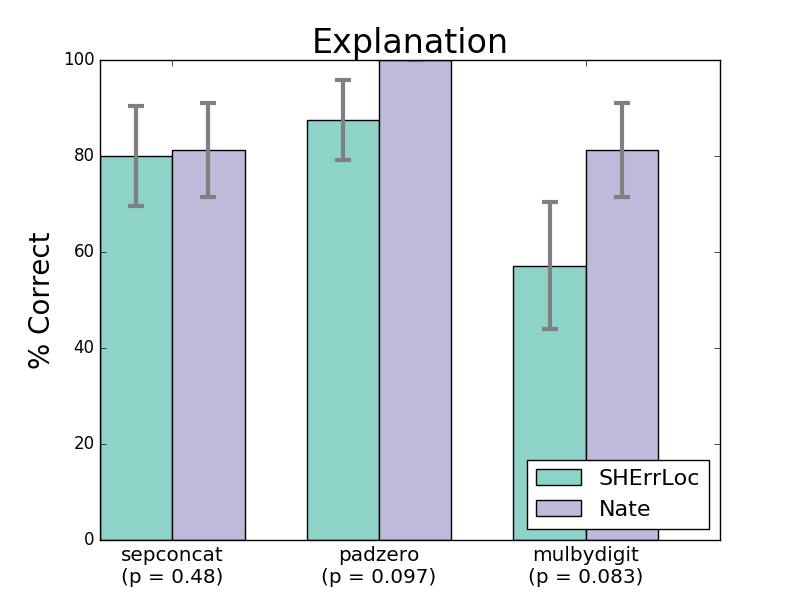
\includegraphics[width=0.7\linewidth]{nate/user-study-reason.png}
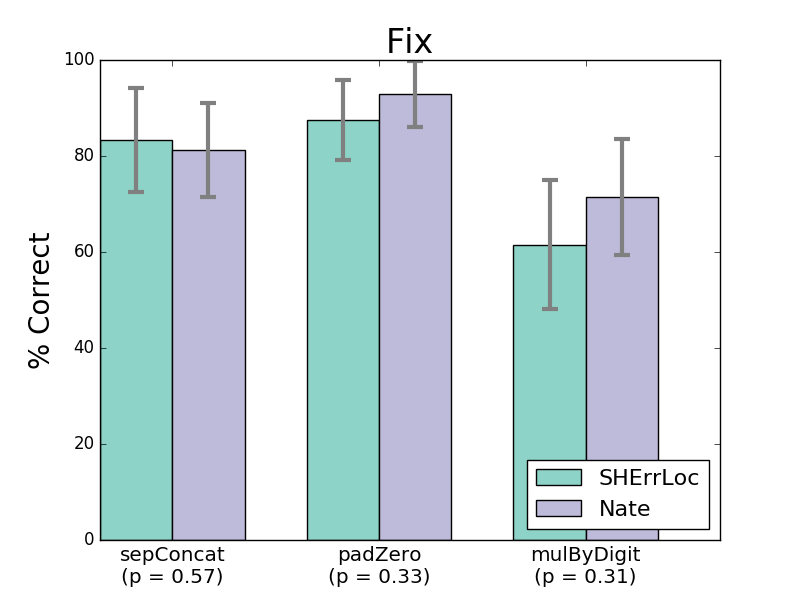
\includegraphics[width=0.7\linewidth]{nate/user-study-fix.png}
% \end{minipage}
% }
% \vspace{3ex}
\caption{A classification of students' explanations and fixes for type
  errors, given either \sherrloc or \toolname's blame assignment.
  %
  The students given \toolname's location generally scored
  better than those given \sherrloc's.
  %
  We report the result of a one-sided Mann-Whitney $U$ test for
  statistical significance in parentheses.}
\label{fig:results-user-study}
\end{figure}

\paragraph{Results}
%
The measured kappa values were $\kappa = 0.68$ for the explanations and
$\kappa = 0.77$ for the fixes; while there is no formal notion for what
consititutes strong agreement~\cite{Krippendorff2012-wd}, kappa values
above $0.60$ are often called ``substantial''
agreement~\cite{Landis1977-ey}.
%
Figure~\ref{fig:results-user-study} summarizes a single annotator's
results, which show that students given \toolname's blame assignment
were generally more likely to correctly explain and fix the type error
than those given \sherrloc's.
%
While there was no discernible difference between \toolname and
\sherrloc for |sepConcat|, \toolname responses for |padZero| and
|mulByDigit| were marked correct 5--30\% more often than the \sherrloc
responses.
%
The results appear to show a trend in favor of \toolname;
%
however, they are not statistically significant so
we cannot discount the possibility of confounding factors.
%


%%% Local Variables:
%%% mode: latex
%%% TeX-master: "main"
%%% End:
